\section{RanggaPutraRamdhani(1174056)}
\subsection{Point Polyline dan Polygon}
\begin{enumerate}
	\item 
	\lstinputlisting{src/1/1174056/py1.py}
	\begin{figure}[H]
		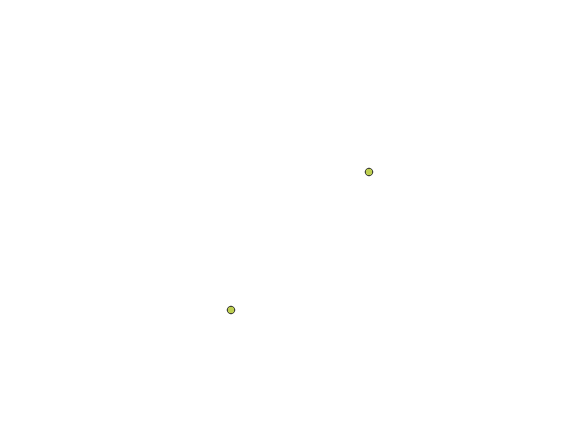
\includegraphics[width=12cm]{figures/1174056/1.PNG}
		\centering
		\caption{Point}
	\end{figure}
	
	\item 
	\lstinputlisting{src/1/1174056/py2.py}
	\begin{figure}[H]
		
\includegraphics[width=12cm]{figures/1174056/2.PNG}
		\centering
		\caption{Point}
	\end{figure}
	
	\item 
	\lstinputlisting{src/1/1174056/py3.py}
	\begin{figure}[H]
		
\includegraphics[width=12cm]{figures/1174056/3.PNG}
		\centering
		\caption{Point}
	\end{figure}
	
	\item 
	\lstinputlisting{src/1/1174056/py4.py}
	\begin{figure}[H]
		
\includegraphics[width=12cm]{figures/1174056/4.PNG}
		\centering
		\caption{Point}
	\end{figure}
	
	\item 
	\lstinputlisting{src/1/1174056/py5.py}
	\begin{figure}[H]
		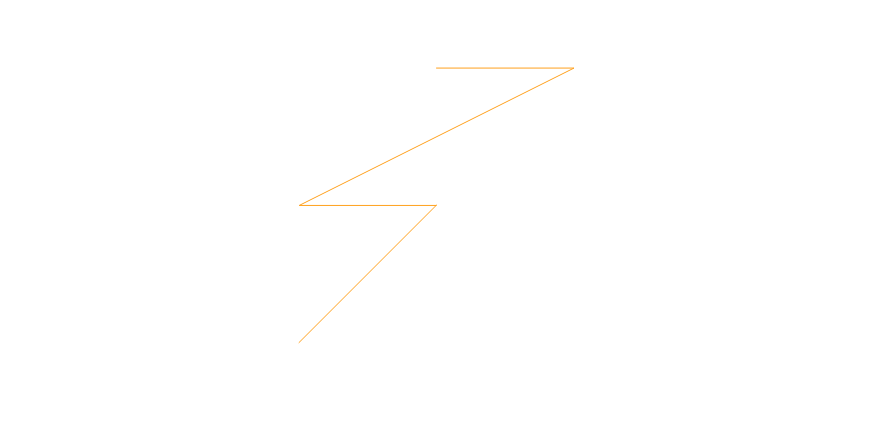
\includegraphics[width=12cm]{figures/1174056/5.PNG}
		\centering
		\caption{Polyline}
	\end{figure}
	
	\item 
	\lstinputlisting{src/1/1174056/py6.py}
	\begin{figure}[H]
		
\includegraphics[width=12cm]{figures/1174056/6.PNG}
		\centering
		\caption{Poligon}
	\end{figure}
	
	\item 
	\lstinputlisting{src/1/1174056/py7.py}
	\begin{figure}[H]
		
\includegraphics[width=12cm]{figures/1174056/7.PNG}
		\centering
		\caption{Polygon}
	\end{figure}
	
	\item 
	\lstinputlisting{src/1/1174056/py8.py}
	\begin{figure}[H]
		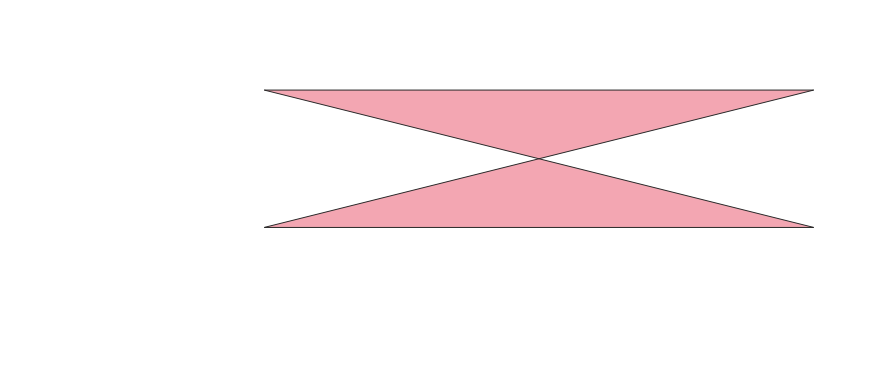
\includegraphics[width=12cm]{figures/1174056/8.PNG}
		\centering
		\caption{Polygon}
	\end{figure}
	
	\item 
	\lstinputlisting{src/1/1174056/py9.py}
	\begin{figure}[H]
		
\includegraphics[width=12cm]{figures/1174056/9.PNG}
		\centering
		\caption{Polygon}
	\end{figure}
	
	\item 
	\lstinputlisting{src/1/1174056/py10.py}
	\begin{figure}[H]
		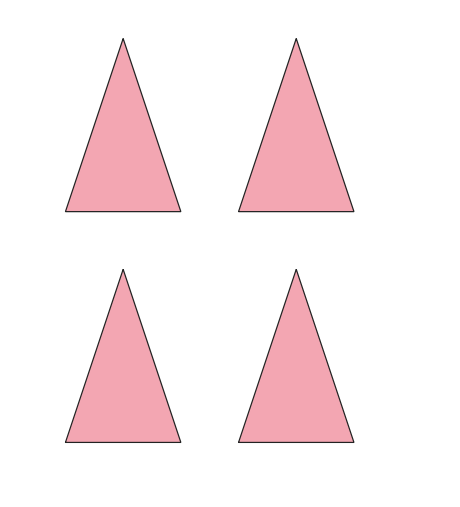
\includegraphics[width=12cm]{figures/1174056/10.PNG}
		\centering
		\caption{Hasil Mod saya 0 berbentuk segitiga sama kaki}
	\end{figure}	
\end{enumerate}

\subsection{Link}
\href{https://youtu.be/5X5gnr74VV4}{Youtube!}